\subsubsection{Regulador con tensión de salida fija}

\begin{figure}[ht]
    \centering
    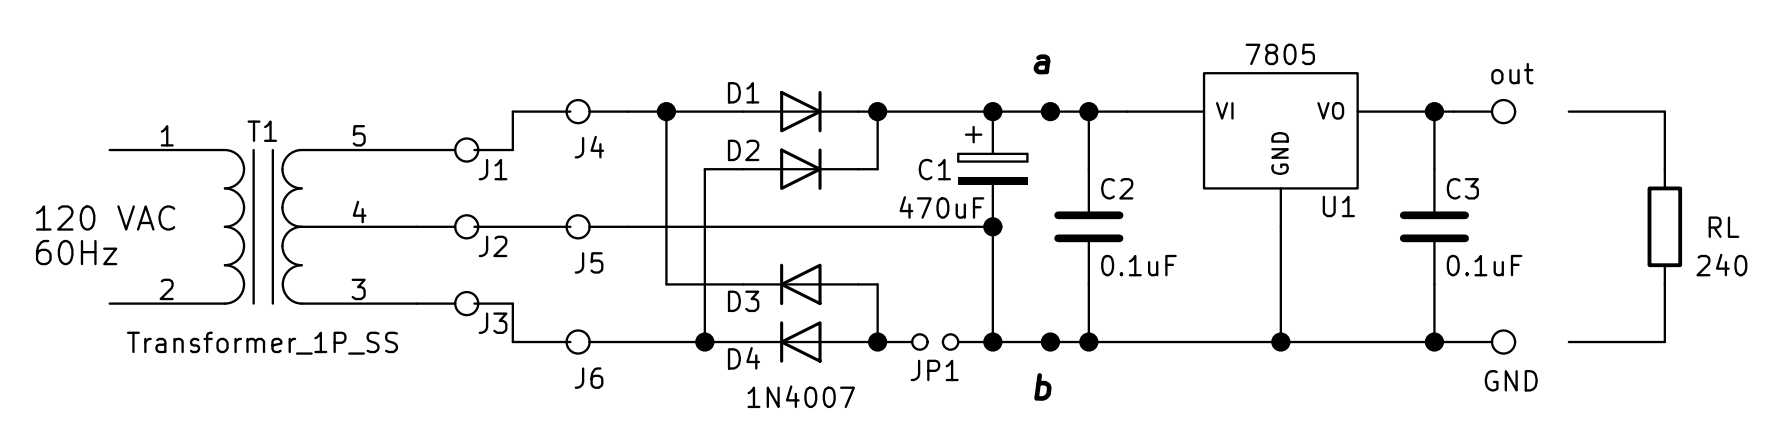
\includegraphics[width=0.8\textwidth]{regulador-tension-salida-fija.png}
    \caption{Regulador lineal con tensión de salida fija}
    \label{fig:regulador-lineal-tension-fija}
\end{figure}

\subsubsection*{Explicar la función de los condensadores $C_2$ y $C_3$ en la figura \ref{fig:regulador-lineal-tension-fija}}

El dispositivo siempre debe estar equipado con un capacitor de entrada para reducir los efectos de la inductancia parásita en los cables de entrada, especialmente si el regulador está ubicado lejos de la fuente no regulada, y un capacitor de salida para ayudar a mejorar la respuesta a los cambios repentinos en la corriente de carga. Para obtener los mejores resultados, use cables y trazos gruesos, mantenga los cables cortos y monte ambos capacitores lo más cerca posible del regulador. Dependiendo del caso, puede ser necesario un disipador de calor para mantener la temperatura interna dentro de niveles tolerables.

\subsubsection*{Explicar cómo conectar el puente de diodos si el transformador no tiene toma central (CT).}

Si el transformador tiene toma central, se deja el jumper $\jumper{1}$ abierto, si no se tiene toma central, se cierra el jumper $\jumper{1}$ y se asegura que en ese nodo haya una referencia.

\subsubsection*{Suponiendo una carga de $80mA$ determine la tensión de rizado pico-pico que se va a presentar en $C_1$}.

Se tiene que el voltaje de rizo pico pico $V_{rpp}$ viene dada por la siguiente ecuación:

\begin{equation}
    V_{rpp} = \frac{I_{cd}}{2 f C}
\end{equation}

teniendo en cuenta que $f= 60Hz$ y $C= 470\mu F$  nos queda.

\begin{align*}
    V_{rpp} &= \frac{80m A}{2 \cdot 60Hz \cdot 470\mu F} \\
    V_{rpp} &= 1.42 V
\end{align*}

\subsubsection*{Determinar la tensión mínima del secundario del transformador en función de la corriente de salida, de manera que el regulador puede mantener la regulación.}

Según los datos del datasheet, la tensión de entrada mínima para mantener la regulación tiene que  ser de $ V_{ir} = 7.5V$. Ahora, para calcular la tensión en el secundario se debe calcular la caida de tensión tomando en cuenta los diodos, el voltaje de riso y el voltaje mínimo del regulador:

\begin{equation}
    V_{s} = 2 V_{d} + V_{rpp} + V_{ir}
    \label{eq:tension-min-secundario}
\end{equation}

$$ V_{s} = 10.32 V $$
 
O si se expresa en rms:

$$ V_{srms} = \frac{V_s}{\sqrt{2}} $$

$$ V_{srms} = 7.30 V $$

\subsubsection*{Determinar la relación que se va a obtener al colocar unas cargas de 100mA}

Recordando que la regulación de voltaje viene dada por:

\begin{equation}
    reg = \frac{V_{cc} - V_{sc}}{V_{sc}} 100 %
\end{equation}

Una carga de $100mA$ viene dada por:

$$ R = \frac{V}{I} = \frac{5V}{100mA} = 50 \Omega $$

Por tanto la regulación de voltaje será:

\begin{equation}
    reg = \frac{5 -5}{5} 100 = 0\%
\end{equation}

\subsubsection{Fuente regulada ajustable}

\begin{figure}[ht]
    \centering
    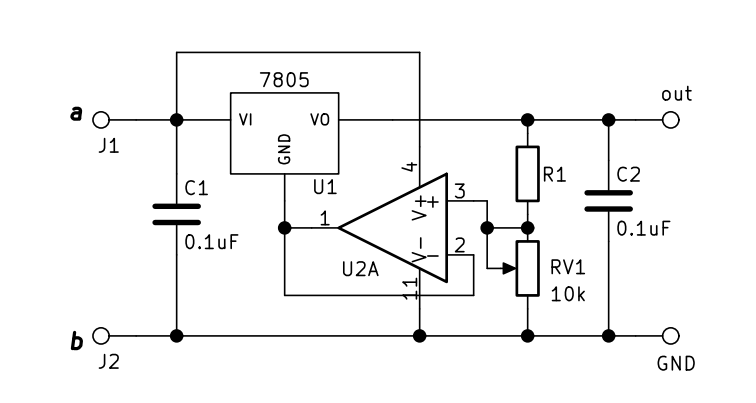
\includegraphics[width=0.8\textwidth]{regulador-tension-salida-ajustable.png}
    \caption{Fuente regulada ajustable}
    \label{fig:regulador-tension-salida-ajustable}
\end{figure}

\subsubsection*{Determinar el rango de tensiones de salida en función del accionamiento <<x>>}

sabemos que:

$$ I = \frac{5 V}{R_1}$$

$$ V_2 = I . x R_{v1}$$

y de la ecuación

\begin{equation}
    V_o = V_1 + I(V_2)
\end{equation}
 
tenemos 

\begin{align*}
    V_o &= 5V + \frac{5 V}{R_1} (x R_{v1}) \\
    V_o &= 5 \WrapParenthesis{1 + \frac{x R_{v1}}{R_{1}}} \\
\end{align*}

los valores de $x$ son $ 0 \leq x \leq 1$ por lo tanto.

\begin{equation}
    5 \leq V_o \leq 5 + \frac{R_{v1}}{R_{1}}
\end{equation}

\subsubsection*{Asignar el valor de $R_1$ de modo que la fuente suministre tensiones de hasta al menos 15V}

Partiendo de la expresión del valor máximo de $V_o$ podemos obtener el valor de $R_1$ que cumple con la condición:

\begin{align*}
    15V &= 5(1 + \frac{R_{v1}}{R_{1}}) \\
    3V &= 1 + \frac{R_{v1}}{R_{1}} \\
    2V &= \frac{R_{v1}}{R_{1}} \\
    R_{1} &= \frac{R_{v1}}{2} \\
    R_{1} &=  \frac{10k}{2} \\
\end{align*}

\begin{equation}
    \boxed{R_{1} = 5k \Omega}
\end{equation}

\subsubsection*{Determinar la corriente de polarización que suministra el amplificador operacional}

La corriente de polarización es la corriente que pasa por la resistencia $R_1$, por lo tanto:

\begin{align*}
    I &= \frac{V}{R_1}  \\
    I &= \frac{5V}{5k \Omega} \\
    I &= 1mA
\end{align*}

\subsubsection*{Determinar la tensión minima de secundario del transformador en función de la corriente de salida, de manera que el regulador pueda mantener la regulación}

Para obtener la tensión mínima del secundario se vuelve a utilizar la ecuación \ref{eq:tension-min-secundario}, está vez sustituyendo $V_{ir}$ por 15V:

\begin{align*}
    V_s &= 15V + \frac{I_{dc}}{2\cdot 60 \cdot 470\cdot 10^{-6}} + 2 \cdot 0.7 V \\
    V_s &= 16.40 + 17.73  I_{dc} \\
\end{align*}

Su valor rms sería:

$$ V_{srms} = \frac{V_s}{\sqrt{2}} $$

$$ V_{srms} = (11.60 + 12.53 I_{dc} )V $$

\subsubsection{Fuente de corriente variable}

\begin{figure}[ht]
    \centering
    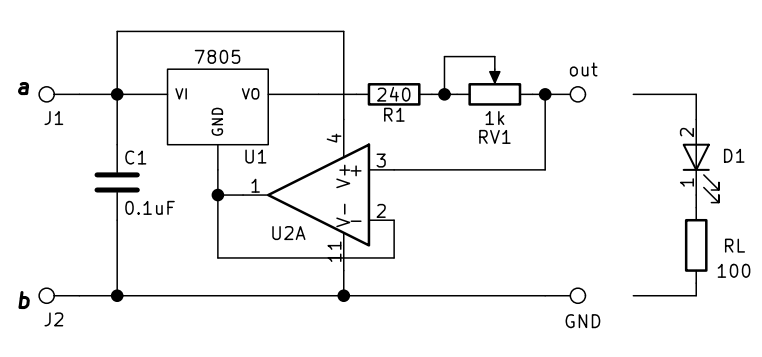
\includegraphics[width=0.8\textwidth]{fuente-corriente-variable.png}
    \caption{Fuente de corriente variable}
    \label{fig:fuente-corriente-variable}
\end{figure}

\subsubsection*{Determinar el rango de corrientes de salida en función del accionamiento <<x>>}

utilizando la relación:

\begin{equation}
    I_o = \frac{5V}{R_1 + xR_{v1}}
\end{equation}

\begin{equation}
    I_o = \frac{5V}{240 \Omega + x 1k \Omega}
\end{equation}

para rangos de $x$ entre $0$ y $1$ se tiene que:

\begin{equation*}
    4.03 mA \leq I_o \leq 20.83 mA 
\end{equation*}

\subsubsection{Simulaciones}

\subsubsection*{Regulador de tensión de salida fija}

\begin{figure}[ht]
    \centering
    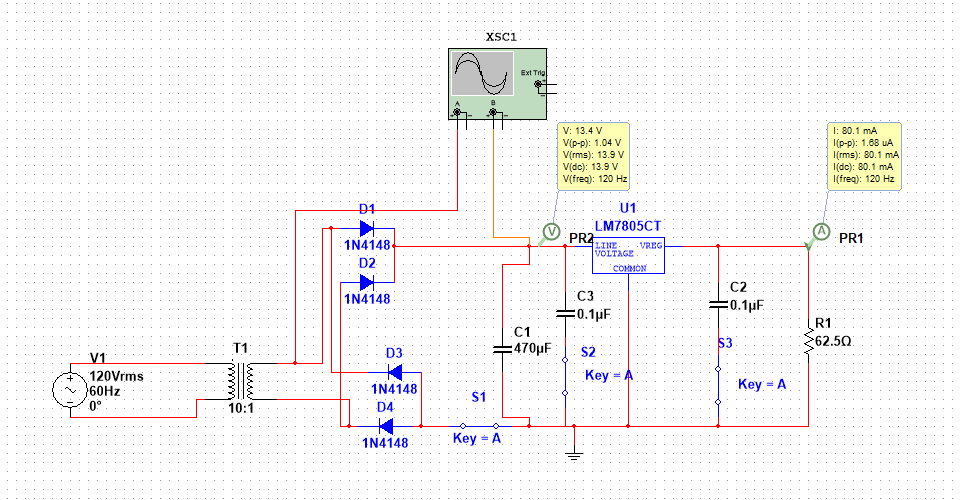
\includegraphics[width=0.8\textwidth]{simulaciones/montaje-regulador-salida-fija-sin-ct.png}
    \caption{Simulación de regulador de tensión fija sin center tap}
    \label{fig:simulacion-regulador-tension-fija-sin-ct}
\end{figure}

La figura \ref{fig:simulacion-regulador-tension-fija-sin-ct} muestra la simulación de un regulador de tensión fija sin center tap, se observa que para una carga de $80mA$ el voltaje de riso es $1.05 Vpp$, el cual es semejante al valor que calculamos $1.42 V$.

Se puede apreciar mejor la forma de la onda de riso en la figura \ref{fig:onda-de-riso-sin-ct} 

\begin{figure}[ht]
    \centering
    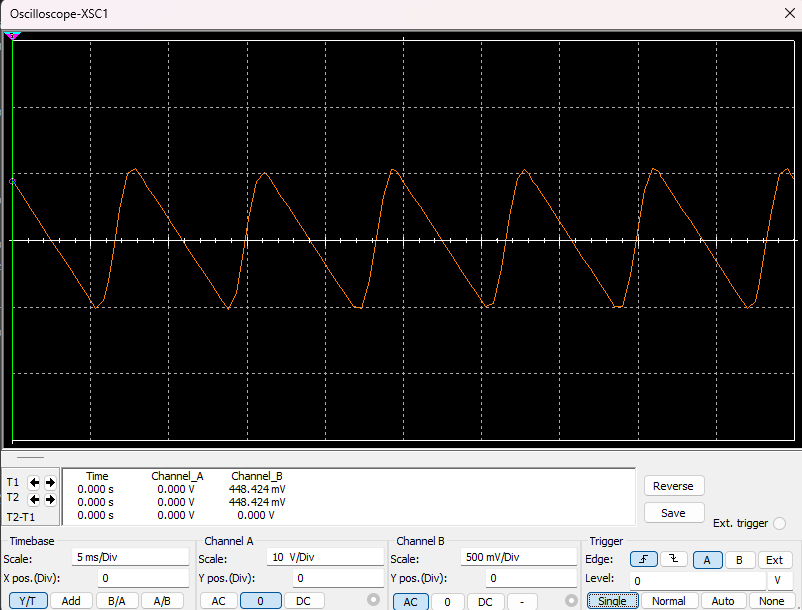
\includegraphics[width=0.6\textwidth]{simulaciones/onda-de-riso-sin-ct.png}
    \caption{Onda de riso sin center tap}
    \label{fig:onda-de-riso-sin-ct}
\end{figure}

En la figura \ref{fig:minima-excursion-regulador-salida-fija} se puede apreciar una comparación entre el voltaje de salida del regulador cuando $V_{srms} > 7.50$ y cuando $V_{srms} < 7.50$. En el primer caso el regulador trabaja con normalidad y podemos observar una tensión de salida sin ruido de $5V$, en el segundo caso podemos observar que el regulador no funciona correctamente y aparece un ruido en la salida debido al efecto riso.

\begin{figure}[ht]
    \centering
    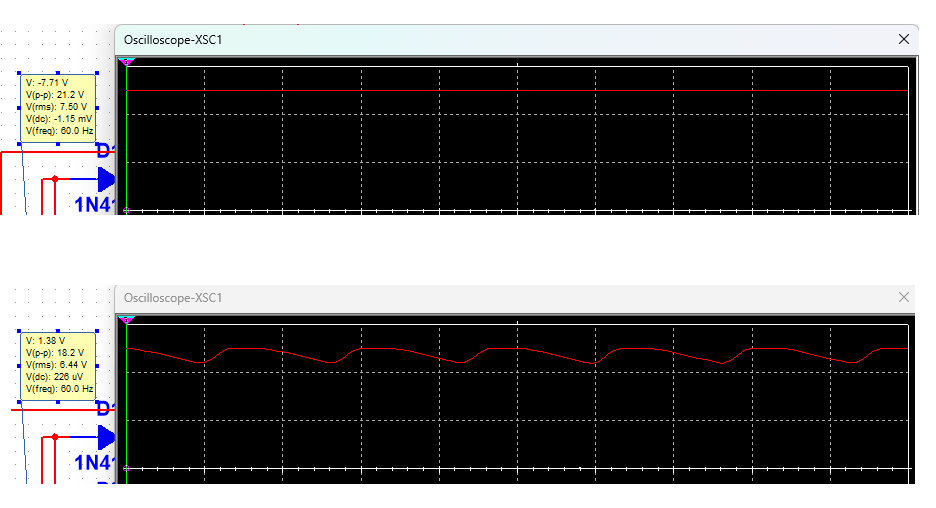
\includegraphics[width=0.8\textwidth]{simulaciones/minima-excursion-regulador-salida-fija.png}
    \caption{Minima excursion regulador de tensión salida fija}
    \label{fig:minima-excursion-regulador-salida-fija}
\end{figure}

En la figura \ref{fig:regulacion-voltaje-regulador-salida-fija} se puede apreciar que para ambos casos (con carga y sin carga) el voltaje es el mismo ($5V$), por lo tanto la regulación de voltaje es 0\%.

\begin{figure}[ht]
    \centering
    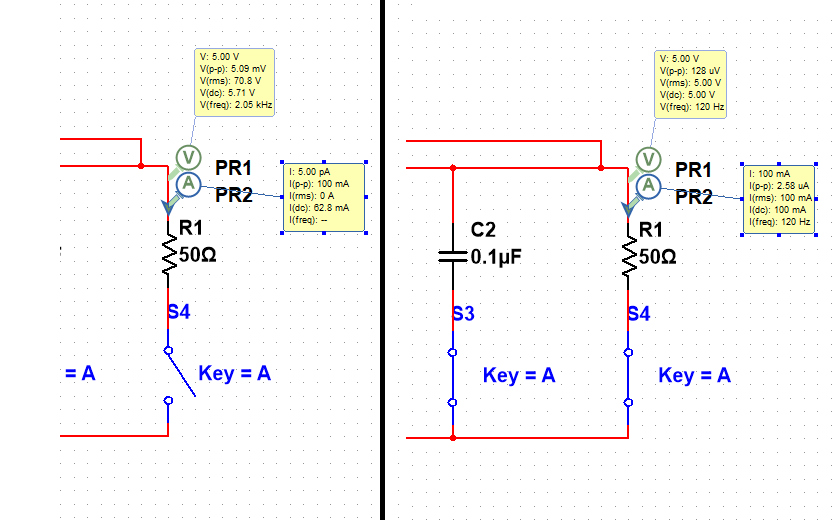
\includegraphics[width=0.8\textwidth]{simulaciones/regulacion-voltaje-regulador-salida-fija.png}
    \caption{Regulación de voltaje del regulador de tensión salida fija}
    \label{fig:regulacion-voltaje-regulador-salida-fija}
\end{figure}

\FloatBarrier
\subsubsection*{Fuente regulada ajustable}

La figura \ref{fig:simulacion-fuente-ajustable} muestra el montaje de una fuente ajustable usando el valor de $R_1 = 5k \Omega$. En esta figura se puede observar que cuando $X=0$ la tensión de salida es $V_0 = 7 V$

\begin{figure}[ht]
    \centering
    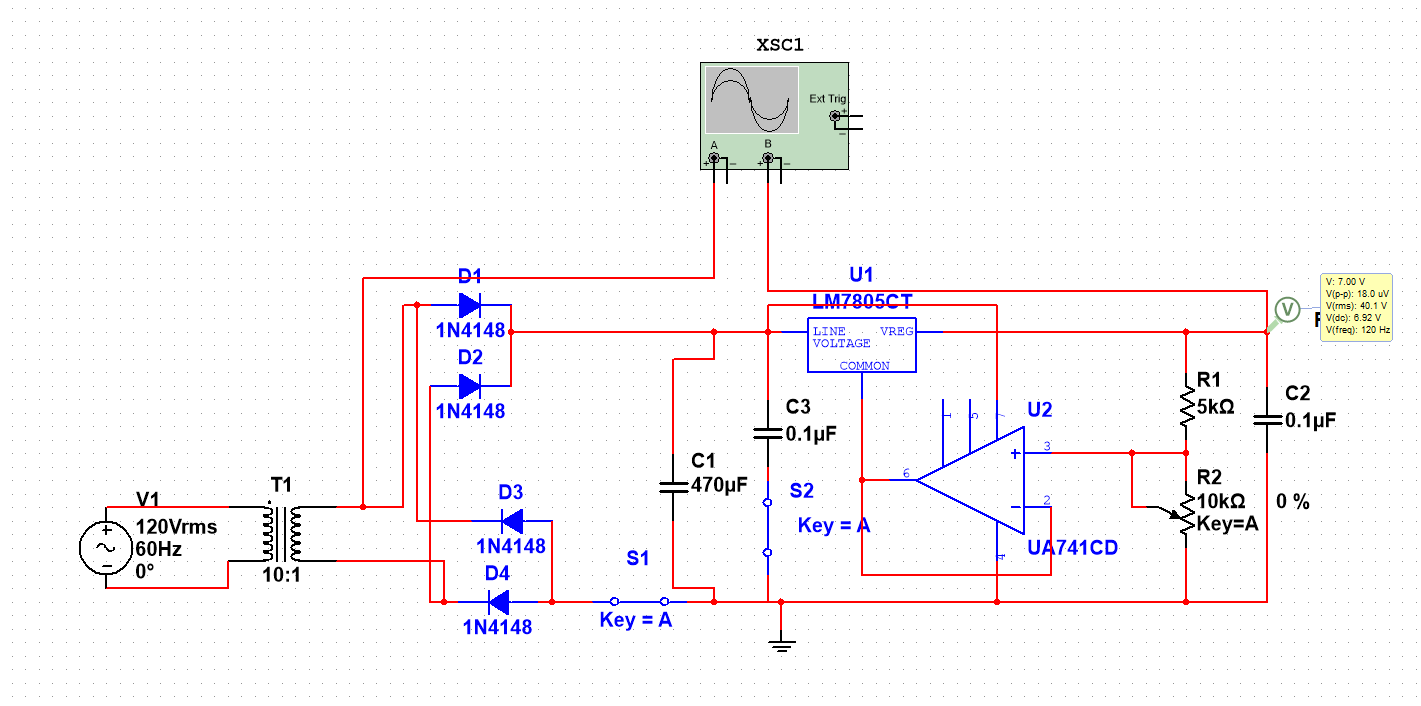
\includegraphics[width=0.8\textwidth]{simulaciones/montaje-regulador-salida-variable.png}
    \caption{Simulación de fuente ajustable}
    \label{fig:simulacion-fuente-ajustable}
\end{figure}

Por otro lado, cuando $X=1$, de la figura \ref{fig:voltaje-salida-max-regulador-ajustable} podemos observar que la tensión de salida es $V_0 = 15.0 V$ que es el valor que se espera para la máxima tensión de salida del regulador de tensión ajustable.

\begin{figure}[ht]
    \centering
    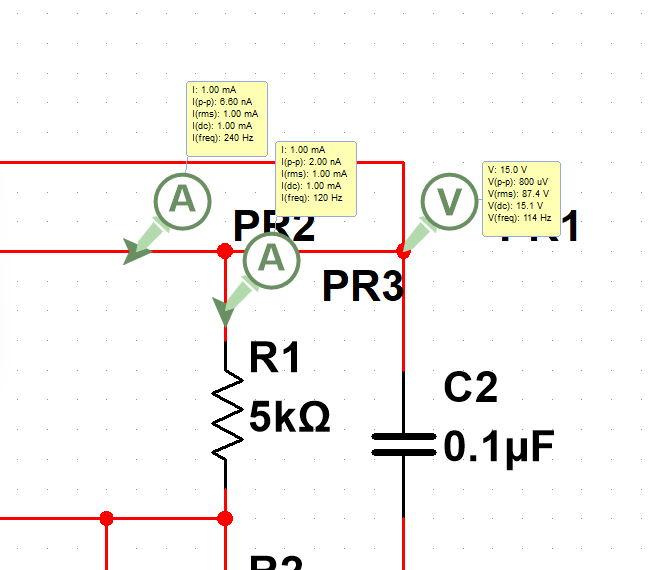
\includegraphics[width=0.5\textwidth]{simulaciones/voltaje-salida-max-regulador-ajustable.png}
    \caption{Voltaje de salida máximo de la fuente ajustable}
    \label{fig:voltaje-salida-max-regulador-ajustable}
\end{figure}

en la figura \ref{fig:corriente-polarizacion-regulador-ajustable} se observa que la corriente a traves de la resistencia $R_1$ es $I = 920 \mu A$.

\begin{figure}
    \centering
    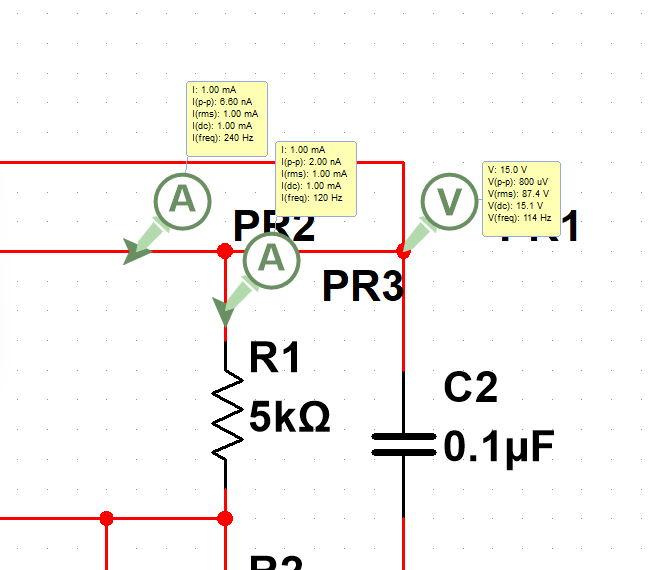
\includegraphics[width=0.6\textwidth]{simulaciones/corriente-polarizacion-regulador-ajustable.png}
    \caption{Corriente de polarización del regulador de tensión ajustable}
    \label{fig:corriente-polarizacion-regulador-ajustable}
\end{figure}

En la figura \ref{fig:minima-excursion-regulador-salida-variable} se observa que cuando la tensión en el secundario del transformador es menor a $11 Vrms$ el regulador no es capaz de suministrar los $15V$ y también se puede observar el ruido del voltaje de riso $V_r$.

\begin{figure}
    \centering
    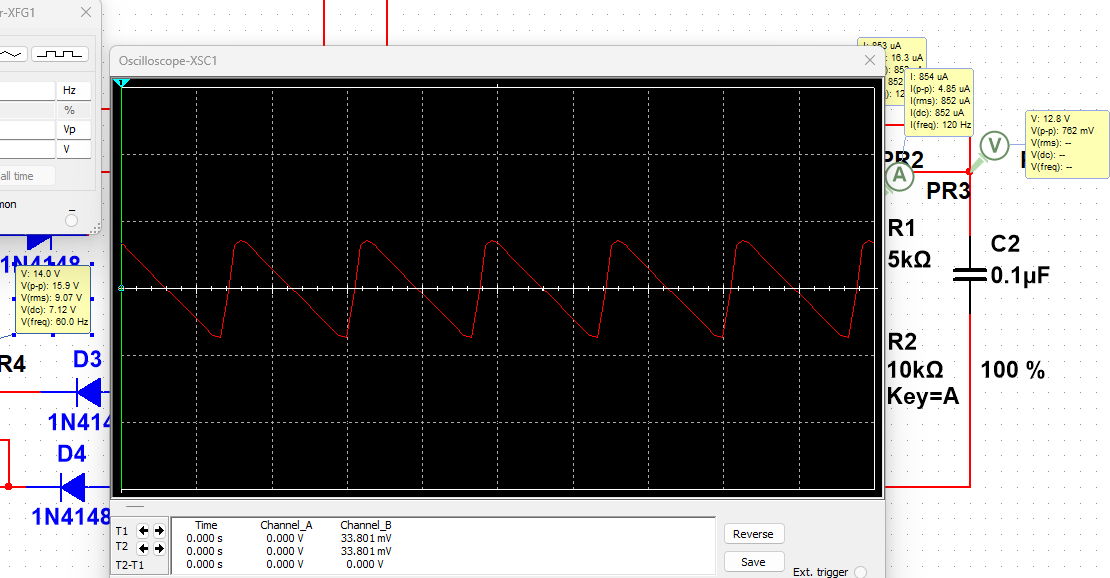
\includegraphics[width=0.6\textwidth]{simulaciones/minima-excursion-regulador-salida-variable.png}
    \caption{Minima excursion regulador de tensión salida variable}
    \label{fig:minima-excursion-regulador-salida-variable}
\end{figure}

\FloatBarrier
\subsubsection*{Fuente de corriente variable}

En la figura \ref{fig:simulacion-fuente-corriente} se puede observar el montaje de la fuente de corriente variable.

\begin{figure}[ht]
    \centering
    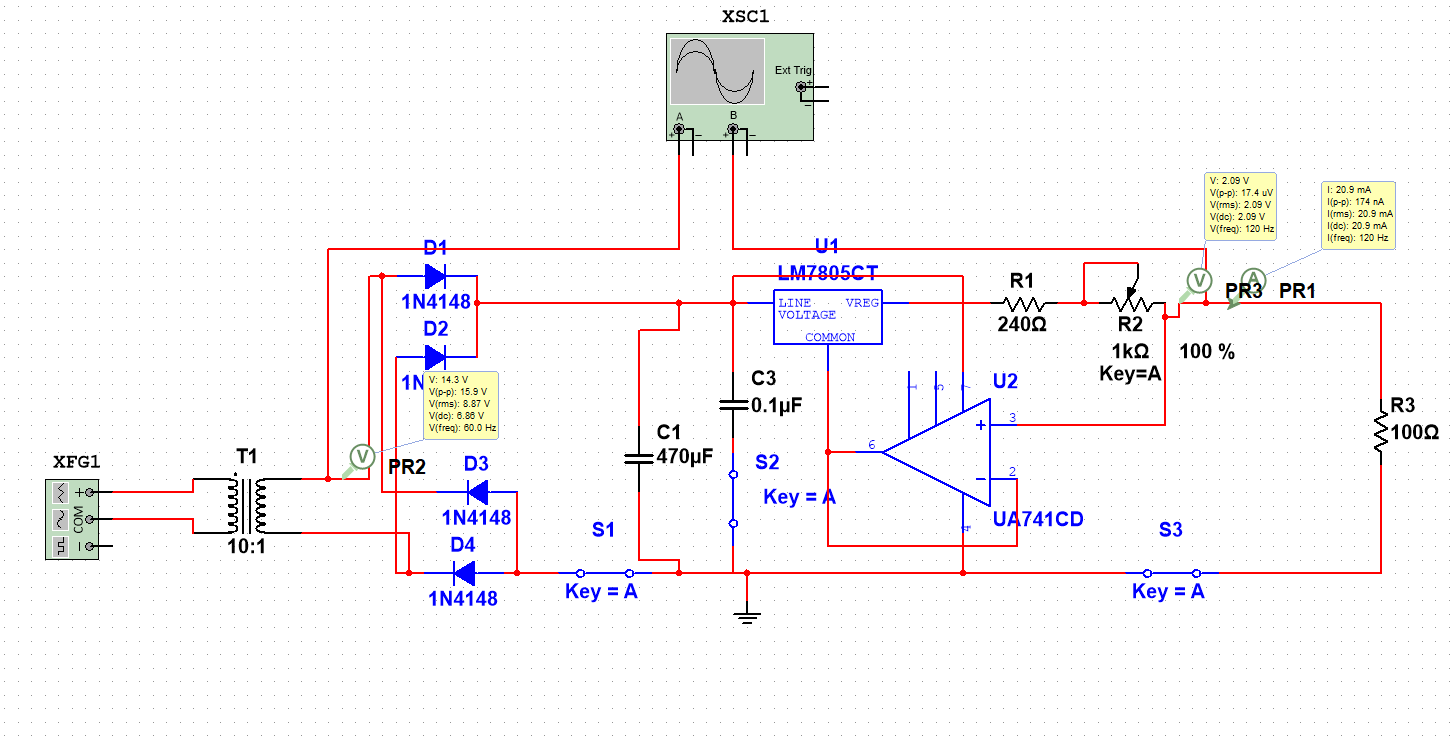
\includegraphics[width=0.8\textwidth]{simulaciones/montaje-fuente-corriente.png}
    \caption{Simulación de fuente de corriente variable}
    \label{fig:simulacion-fuente-corriente}
\end{figure}

En la figura \ref{fig:rango-corriente-salida}, se puede observar una comparativa de la corriente de salida mínima y máxima.

Cuando $x=0$, $I_o = 5.58 mA$ y cuando $x=1$, $I_o = 20.9mA$.

\begin{figure}[ht]
    \centering
    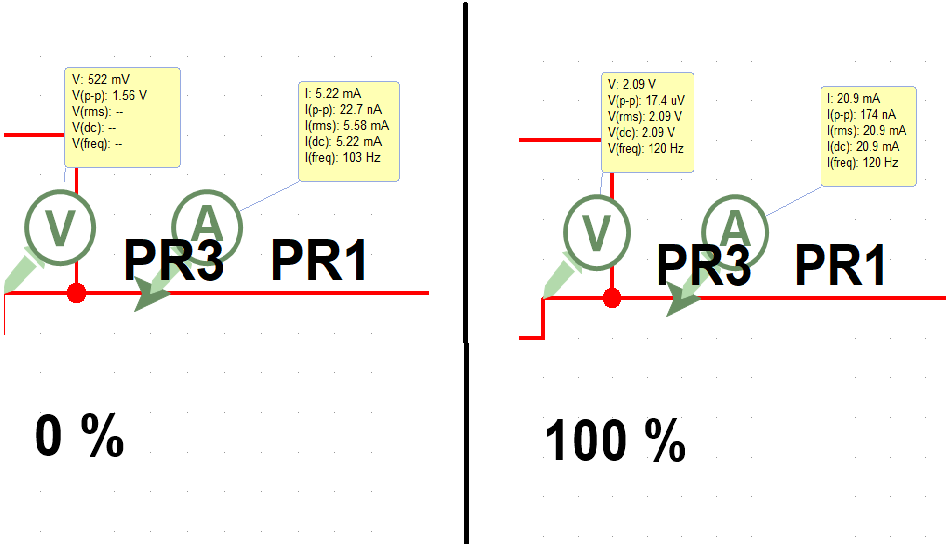
\includegraphics[width=0.8\textwidth]{simulaciones/rango-corriente-salida.png}
    \caption{Comparación corriente de salida minima y máxima}
    \label{fig:rango-corriente-salida}
\end{figure}

\subsubsection{Procedimiento ensayo de laboratorio}

\subsubsection*{Rectificador de tensión}

\begin{enumerate}
    \item Se realiza el montaje de la etapa del rectificador de onda completa y filtro capacitivo.
    \item en caso de contar con center tap, se deja el jumper $\jumper{1}$ abierto, si no se tiene toma central, se cierra el jumper $\jumper{1}$ y se asegura que en ese nodo haya una referencia.
    \item se conecta el primario del transformador a la toma de la mesa de trabajo y el secundario del transformador a los puntos $J_1$, $J_3$ y $j_2$ en caso de contar con center tap.
    \item se conecta la referencia del osciloscopio al nodo b.
\end{enumerate}

\subsubsection*{Regulador de tensión de salida fija}

\begin{enumerate}
    \item Se realiza el montaje del circuito de la figura \ref{fig:regulador-lineal-tension-fija}
    \item se coloca una carga de $68 \Omega$, luego se mide y se fotografía la tensión de riso en el condensador $C1$ 
    \item se coloca el transformador de manera que suministre más de $7Vrms$ y se mide y fotografía, el voltaje de salida del regulador.
    \item se repite el paso anterior, esta vez con el transformador suministrando menos de $7Vrms$.
    \item Ahora se quita la carga y se mide la tensión de salida, para luego colocar una carga de $50 \Omega$ y se vuelve a medir la tensión de salida.
\end{enumerate}

\subsubsection*{Regulador de tensión de salida variable}

\begin{enumerate}
    \item Se realiza el montaje del circuito de la figura \ref{fig:regulador-tension-salida-ajustable}
    \item se ajusta el potenciómetro al mínimo ($x = 0$) y se mide la tensión de salida.
    \item se ajusta el potenciómetro al máximo ($x = 1$) y se mide la tensión de salida.
    \item Se mide la diferencia de tensión entre la resistencia $R_1$ (una medición a cada lado de la resistencia).
    \item se coloca el transformador de manera que suministre más de $12Vrms$ y se mide y fotografía, el voltaje de salida del regulador.
    \item se repite el paso anterior, esta vez con el transformador suministrando menos de $12Vrms$.
\end{enumerate}

\subsubsection*{Fuente de corriente variable}

\begin{enumerate}
    \item Se realiza el montaje del circuito de la figura \ref{fig:fuente-corriente-variable}
    \item se conecta la carga de $100 \Omega$.
    \item se ajusta el potenciómetro al mínimo ($x = 0$) y se mide la tensión de salida (debería dar $I= 4.4 mA$).
    \item se ajusta el potenciómetro al máximo ($x = 1$) y se mide la tensión de salida (debería dar $I= 20.9 mA$).
\end{enumerate}